\chapter{Survival Data and the Kaplan-Meier Curve \label{chapter:km}}

We have already investigated supervised learning models and hypothesis tests in cases where the outcome of interest is a category or number. But what if the outcome is a \emph{time duration}? For example, what if we're comparing the effects of two treatments and our outcome is the time between treatment administration and disease progression?

Data where the outcome is a time duration are very common in clinical data science and are called \textbf{time-to-event} data or \textbf{survival data}. The field of \textbf{survival analysis} develops methods to analyze and interpret such data. We will examine one such method today and many more in subsequent chapters.

%%%%%%%%%%%%%%%%%%%%%%%%%%%%%%%%%%%%%%%%%%%%%%%%%%%%%%%%%%%%%%%%%%%%%%%%%%%%%%%%%%

\section{Example: Ovarian Cancer Survival Dataset}

Today we'll examine some data from a study of ovarian cancer\footnote{The dataset comes from the \texttt{survival} package in R and is labeled \texttt{ovarian}. The original study is Edmonson JH \emph{et al}, ``Different chemotherapeutic sensitivities and host factors affecting prognosis in advanced ovarian carcinoma versus minimal residual disease'', \emph{Cancer Treatment Reports}, 63(2): 241-247; 1979.}. The dataset contains information on $26$~women. The variables are:

{\small
\begin{itemize}
\item \texttt{futime}: The number of days from enrollment in the study until death or censoring, whichever came first
\item \texttt{fustat}: An indicator of death (1) or censoring (0)
\item \texttt{age}: The patient's age in years at the time of treatment administration
\item \texttt{resid.ds}: Residual disease present at the time of treatment administration (1 = no, 2 = yes)
\item \texttt{rx}: Treatment group (1 = cyclophosphamide, 2 = cyclophosphamide + adriamycin)
\item \texttt{ecog.ps}: A measure of performance score or functional status at the time of treatment administration, using the Eastern Cooperative Oncology Group's (ECOG) scale. It ranges from 0 (fully functional) to 4 (completely disabled). Level 4 subjects are usually considered too ill to enter a randomized trial such as this. The patients in this dataset are all at Levels 1 and 2. 
\end{itemize}
}

\noindent Here is a histogram of the follow-up times (\texttt{futime}) in days, colored according to whether the patient died or was censored (\texttt{fustat}):

\begin{center}
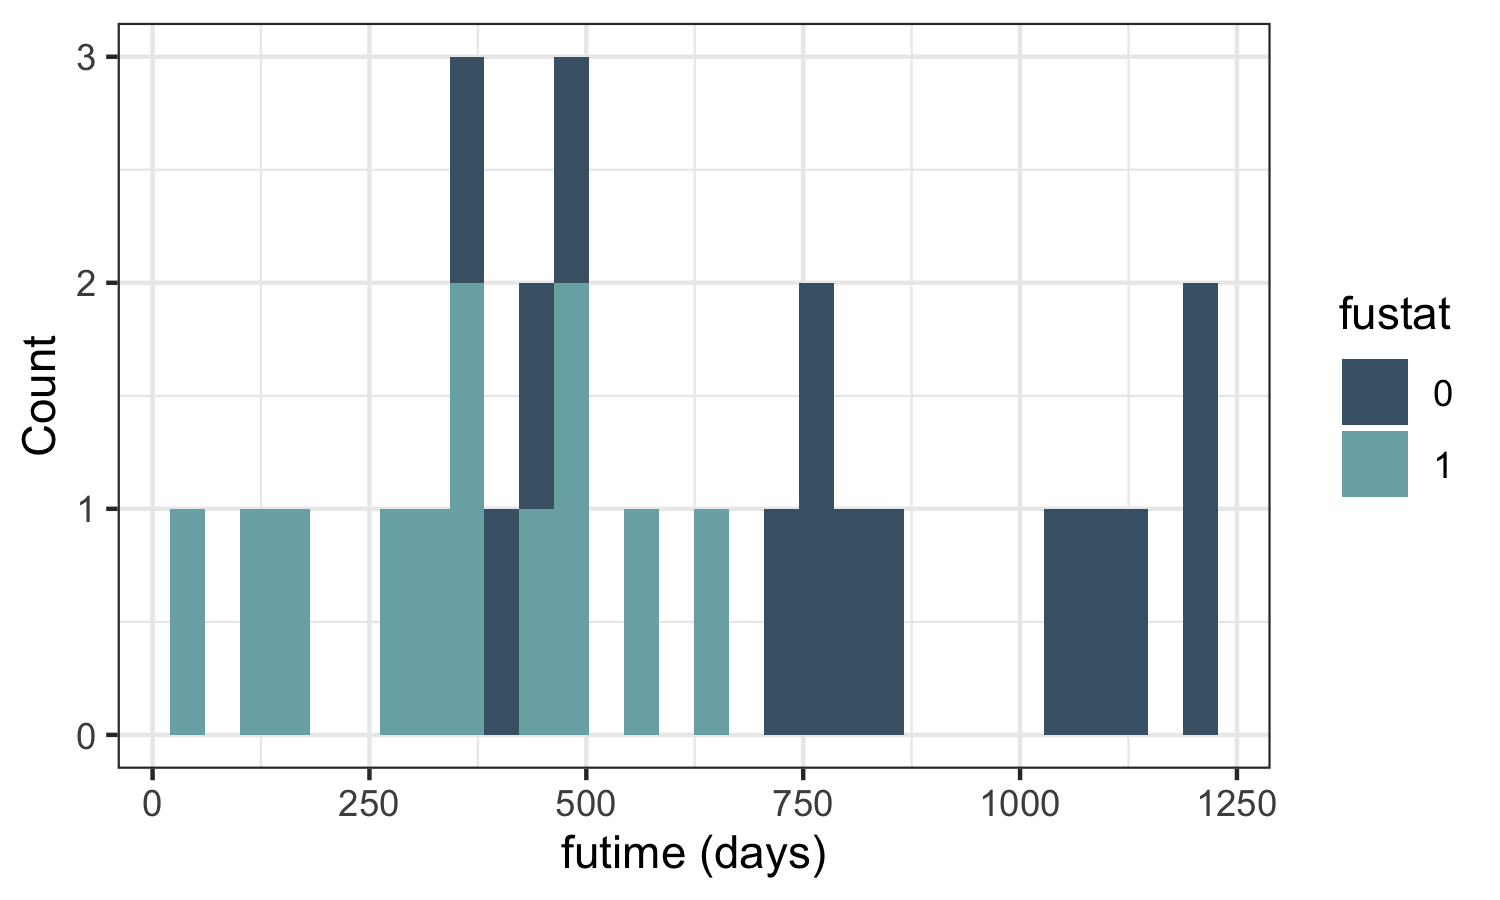
\includegraphics[width=0.7\textwidth]{img/cs-ovarian-futime.png}
\end{center}

\noindent And here is the same graph colored by treatment group (\texttt{rx}):

\begin{center}
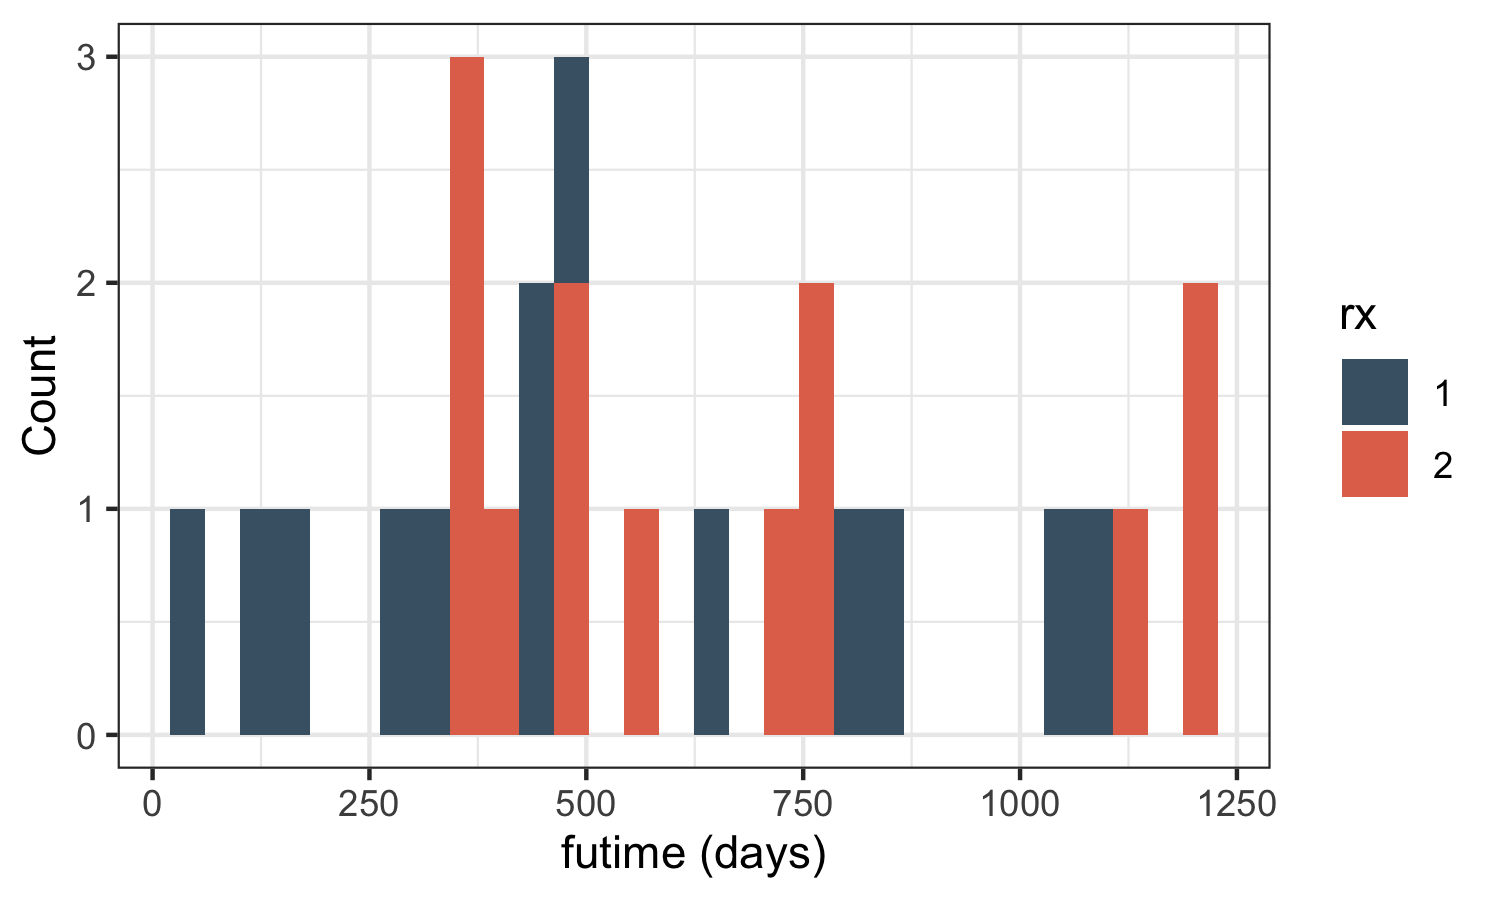
\includegraphics[width=0.7\textwidth]{img/cs-ovarian-futime2.png}
\end{center}

Now, imagine that we want to study the effect of the treatment group (\texttt{rx}) on the outcome of death or no death (1 = death, 0 = no death). We could think of this as a classification problem with only a single feature: treatment group. Unfortunately, this method of analyzing time-dependent data is fraught with problems:

\begin{enumerate}
\item How do you choose the time horizon at which to evaluate mortality?
\item How do you handle people who dropped out of the study before that time?
\end{enumerate}

%%%%%%%%%%%%%%%%%%%%%%%%%%%%%%%%%%%%%%%%%%%%%%%%%%%%%%%%%%%%%%%%%%%%%%%%%%%%%%%%%%

\section{Definitions}

\textbf{Censoring} occurs when the event of interest in a time-to-event analysis is not observed. It is a form of missing data problem (see Chapter~\ref{chapter:missingdata}) and can be caused by a variety of factors, including inconsistencies in follow-up, the study's ending before all subjects have experienced the event, or a lack of knowledge about when, exactly, the event occurred. The type of censoring represented in the \texttt{ovarian} dataset is called \textbf{right-censoring}. We will focus on right-censoring today and investigate other types later.
\begin{quote}
\textbf{Right censoring:} A situation that arises when the event of interest has not occurred by the end of the follow-up period. This may be because (a) the study itself ends, (b) a patient is lost to follow-up during the study period, or (c) a patient experiences a different event that makes further follow-up impossible\footnote{For more information, please see Clark TG \emph{et al}, ``Survival Analysis Part I: Basic Concepts and First Analyses'', \emph{British Journal of Cancer}, 89, 232--238; 2003.}.
\end{quote}

Survival data are generally described using two probabilities, called the survival and hazard. 
\begin{quote}
\textbf{Survival:} Also called the \textbf{survival function} or \textbf{survival probability} and abbreviated $S(t)$, this is the probability that an individual survives to time $t$ (i.e., does not experience the event by time $t$).\\[5mm]
\textbf{Hazard:} Usually denoted by $h(t)$ or $\lambda(t)$, this is the probability that an individual who has not yet experienced the event at time $t$ experiences it at that exact time. In other words, it is the instantaneous event rate for an individual who has already survived to time $t$. 
\end{quote}

We will focus on the survival function now and learn more about the hazard later. 

%%%%%%%%%%%%%%%%%%%%%%%%%%%%%%%%%%%%%%%%%%%%%%%%%%%%%%%%%%%%%%%%%%%%%%%%%%%%%%%%%%

\section{The Kaplan-Meier Estimator}

The \textbf{Kaplan-Meier estimator} is a nonparametric estimate of the survival function, usually represented graphically by a \textbf{Kaplan-Meier curve}\footnote{It can be shown mathematically that the Kaplan-Meier estimator is the maximum likelihood estimator (see Chapter~\ref{chapter:mlebasics}) of the survival function in the case of censoring.}. The Kaplan-Meier estimator looks like this:
$$ \hat{S}(t) = \prod_{j|t_j \leq t} \frac{n_j - d_j}{n_j} $$
where $d_j$ is the number of subjects who fail at time $t_j$ and $n_j$ is the number of subjects at risk just prior to $t_j$. Here is a Kaplan-Meier curve for the \texttt{ovarian} dataset. The little ``+'' signs correspond to censoring events.
\begin{center}
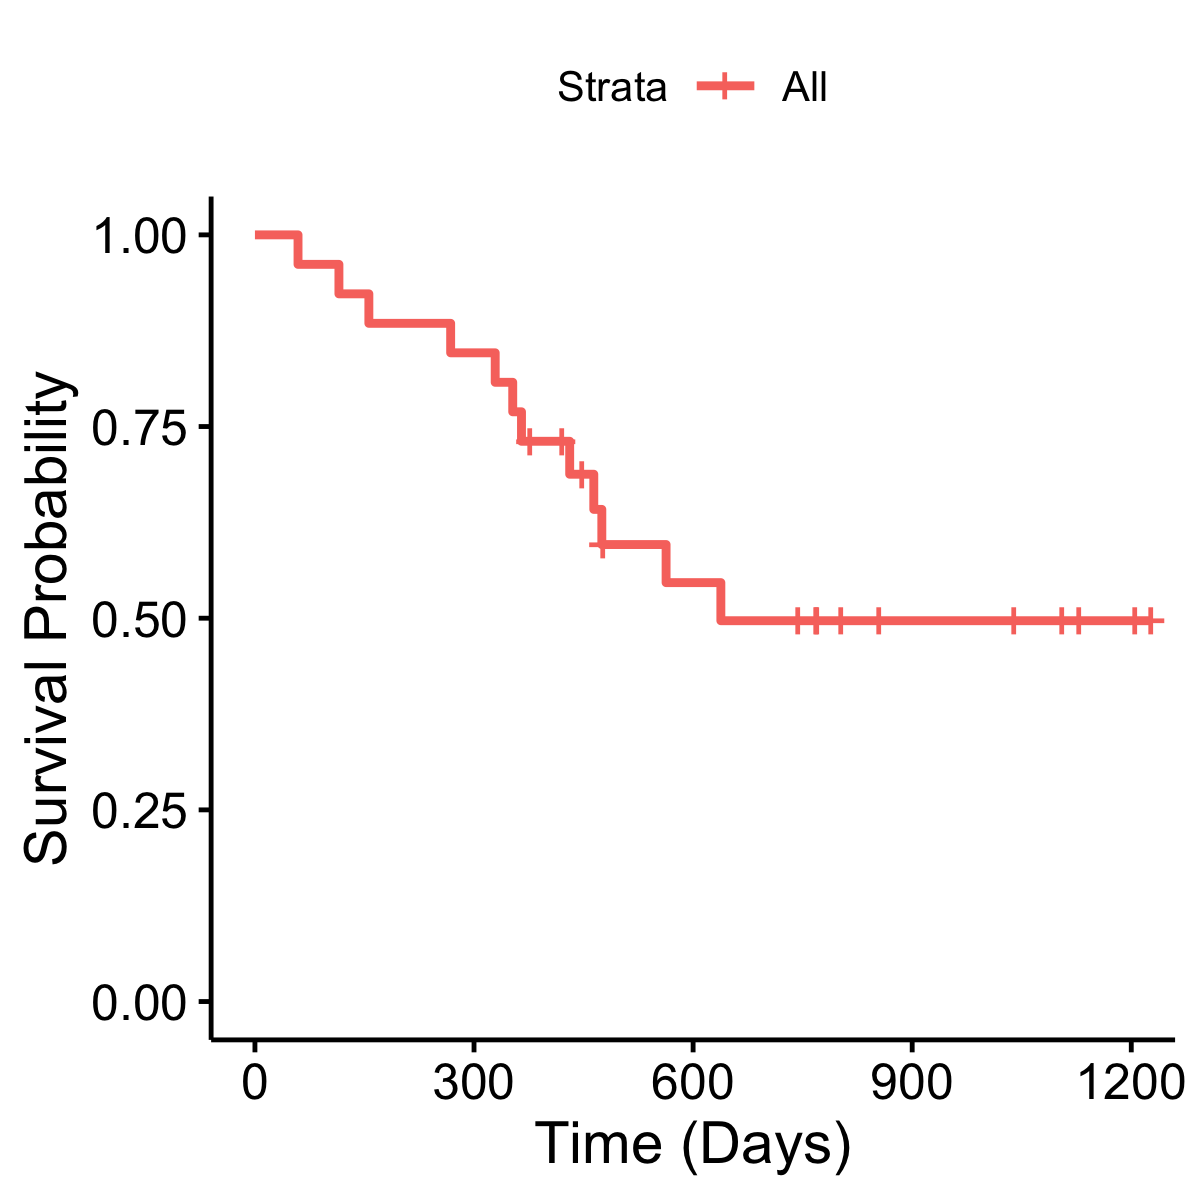
\includegraphics[width=0.6\textwidth]{img/ovarian-km-curve.png}
\end{center}
And here are Kaplan-Meier curves for the two treatment groups separately:
\begin{center}
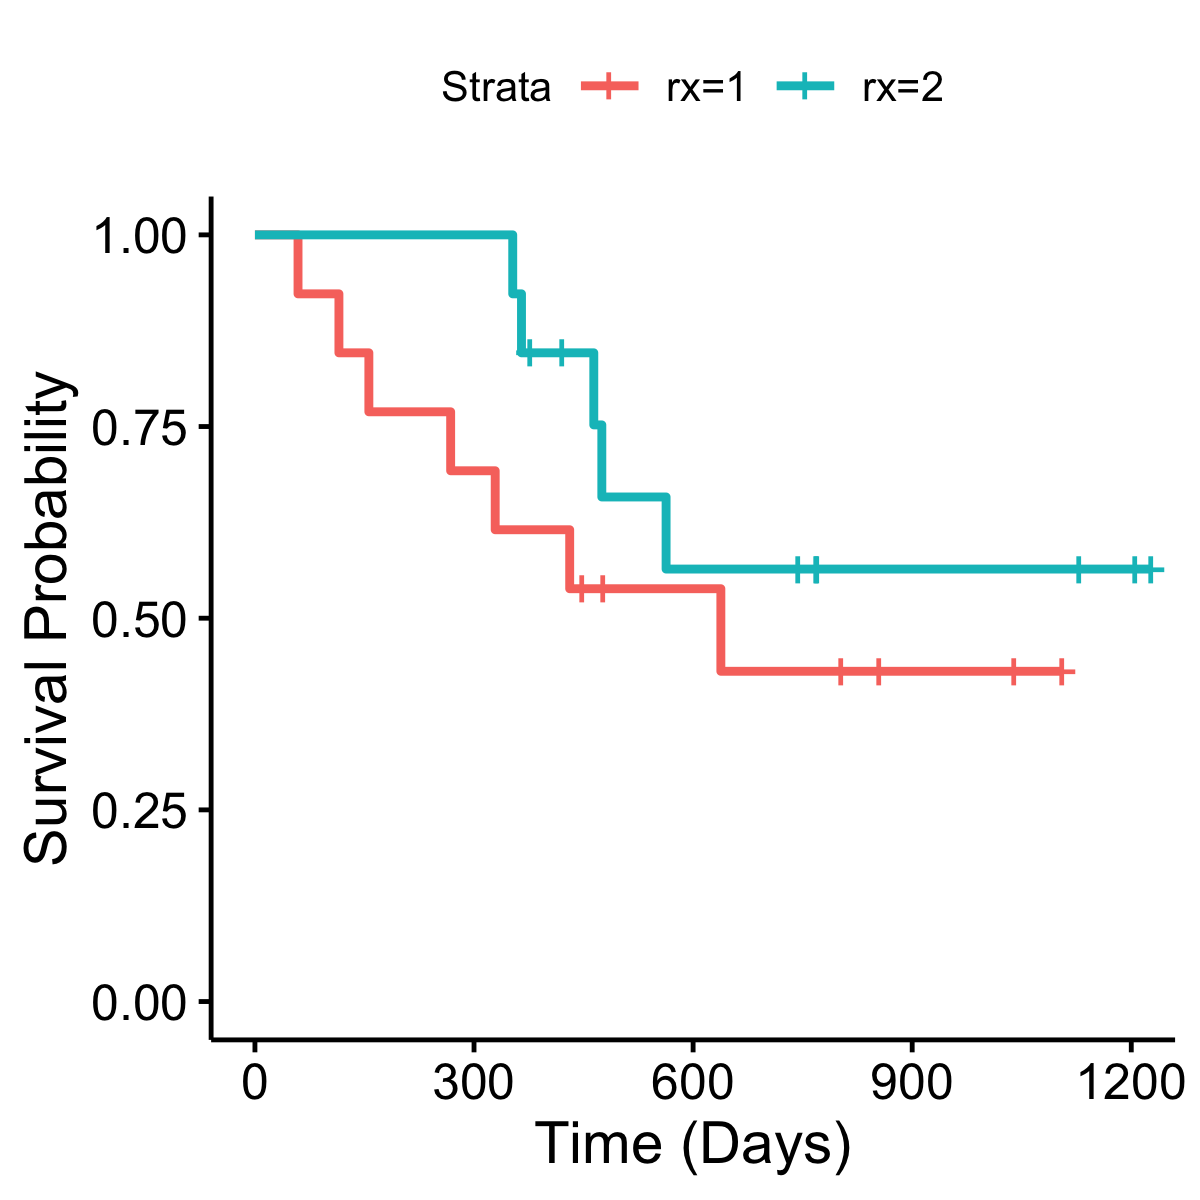
\includegraphics[width=0.6\textwidth]{img/ovarian-km-curve-rx.png}
\end{center}
\vspace{5mm}

\begin{question}{}
Here are the raw data from treatment group $1$ of the \texttt{ovarian} dataset. Using these data, fill in the remaining cells of the table below.
{\small
\begin{center}
\begin{tabular}{rlrr}
  \toprule
 & rx & futime & fustat \\ 
  \midrule
  1 & 1 & 59 & 1 \\ 
  2 & 1 & 115 & 1 \\ 
  3 & 1 & 156 & 1 \\ 
  4 & 1 & 268 & 1 \\ 
  5 & 1 & 329 & 1 \\ 
  6 & 1 & 431 & 1 \\ 
  7 & 1 & 448 & 0 \\ 
  8 & 1 & 477 & 0 \\ 
  9 & 1 & 638 & 1 \\ 
  10 & 1 & 803 & 0 \\ 
  11 & 1 & 855 & 0 \\ 
  12 & 1 & 1040 & 0 \\ 
  13 & 1 & 1106 & 0 \\ 
  \bottomrule
\end{tabular}
\end{center}
}
\vspace{-5mm}
{\small
\begin{center}
\begin{tabular}{rrrrll}
  \toprule
$j$ & $t_j$ & $n_j$ & $d_j$ & $\hat{S}(t_j)$ & Calculation \\ 
  \midrule
  0 & 0 & 13 & 0 & $1.000$ & $\frac{13-0}{13}$ \\
  1 & 59 & 13 & 1 & $0.923$ & $\hat{S}(t_0) \left(\frac{13-1}{13}\right)$ \\
  2 & 115 & 12 & 1 & $0.846$ & $\hat{S}(t_1) \left(\frac{12-1}{12}\right)$ \\[2mm]
  3 & 156 & \\[2mm] % 11 & 1 & $0.769$ & $\hat{S}(t_2) \left(\frac{11-1}{11}\right)$ \\
  4 & 268 & \\[2mm] % 10 & 1 & $0.692$ & $\hat{S}(t_3) \left(\frac{10-1}{10}\right)$ \\
  5 & 329 & 9 & 1 & $0.615$ & $\hat{S}(t_4) \left(\frac{9-1}{9}\right)$ \\
  6 & 431 & 8 & 1 & $0.538$ & $\hat{S}(t_5) \left(\frac{8-1}{8}\right)$ \\
  7 & 448 & 7 & 0 & $0.538$ & $\hat{S}(t_6) \left(\frac{7-0}{7}\right)$ \\
  8 & 477 & 6 & 0 & $0.538$ & $\hat{S}(t_7) \left(\frac{6-0}{6}\right)$\\
  9 & 638 & 5 & 1 & $0.431$ & $\hat{S}(t_8) \left(\frac{5-1}{5}\right)$\\[2mm]
  10 & 803 & 4 & 0 & \\[2mm] % $0.431$ & $\hat{S}(t_9) \left(\frac{4-0}{4}\right)$ \\
  11 & 855 & 3 & 0 & \\[2mm] % $0.431$ & $\hat{S}(t_10) \left(\frac{3-0}{3}\right)$ \\
  12 & 1040 & 2 & 0 & \\[2mm] % $0.431$ & $\hat{S}(t_11) \left(\frac{2-0}{2}\right)$ \\
  13 & 1106 & 1 & 0 & \\[2mm] % $0.431$ & $\hat{S}(t_12) \left(\frac{1-0}{1}\right)$ \\
  \bottomrule
\end{tabular}
\end{center}
}
\end{question}

\begin{question}{}
Based solely on the Kaplan-Meier curves for the two treatment groups, which treatment appears to prolong survival more effectively?
\end{question}

%%%%%%%%%%%%%%%%%%%%%%%%%%%%%%%%%%%%%%%%%%%%%%%%%%%%%%%%%%%%%%%%%%%%%%%%%%%%%%%%%%

\section{Assumptions of the Kaplan-Meier Estimator}

The Kaplan-Meier estimator makes three important assumptions:
\begin{enumerate}
\item The probability of censoring is unrelated to the outcome of interest.
\item The survival probabilities are the same for participants recruited at different times during the study (e.g., circumstances that could alter the survival, such as treatments, do not change over calendar time).
\item The events occurred at exactly the times specified. 
\end{enumerate}

\begin{question}{}
What is one way each of these assumptions could be violated?
\end{question}

%%%%%%%%%%%%%%%%%%%%%%%%%%%%%%%%%%%%%%%%%%%%%%%%%%%%%%%%%%%%%%%%%%%%%%%%%%%%%%%%%%

\section{Comparing Kaplan-Meier Curves}

Of course, now the question arises: How do we formally compare two Kaplan-Meier curves? There is a nonparametric hypothesis test for comparing Kaplan-Meier curves called the log-rank test; we will see it in Chapter~\ref{chapter:hypothesisii}. There is also an entire family of linear models, called Cox proportional hazards models, that use the Kaplan-Meier curve as their backbone and model the effects of different covariates on this curve. We will see them in Chapter~\ref{chapter:cox}.
\vspace{5mm}

\begin{question}{}
Here are the data for treatment group $2$ of the \texttt{ovarian} dataset. Perform the calculations of $\hat{S}(t_j)$ for $j = 0, \dots, 13$, starting with $t_0 = 0$. Draw the Kaplan-Meier curve, adding symbols for the censoring events.
{\small
\begin{center}
\begin{tabular}{rlrr}
  \toprule
 & rx & futime & fustat \\ 
  \midrule
  1 & 2 & 353 & 1 \\ 
  2 & 2 & 365 & 1 \\ 
  3 & 2 & 377 & 0 \\ 
  4 & 2 & 421 & 0 \\ 
  5 & 2 & 464 & 1 \\ 
  6 & 2 & 475 & 1 \\ 
  7 & 2 & 563 & 1 \\ 
  8 & 2 & 744 & 0 \\ 
  9 & 2 & 769 & 0 \\ 
  10 & 2 & 770 & 0 \\ 
  11 & 2 & 1129 & 0 \\ 
  12 & 2 & 1206 & 0 \\ 
  13 & 2 & 1227 & 0 \\ 
  \bottomrule
\end{tabular}
\end{center}
}
\begin{center}
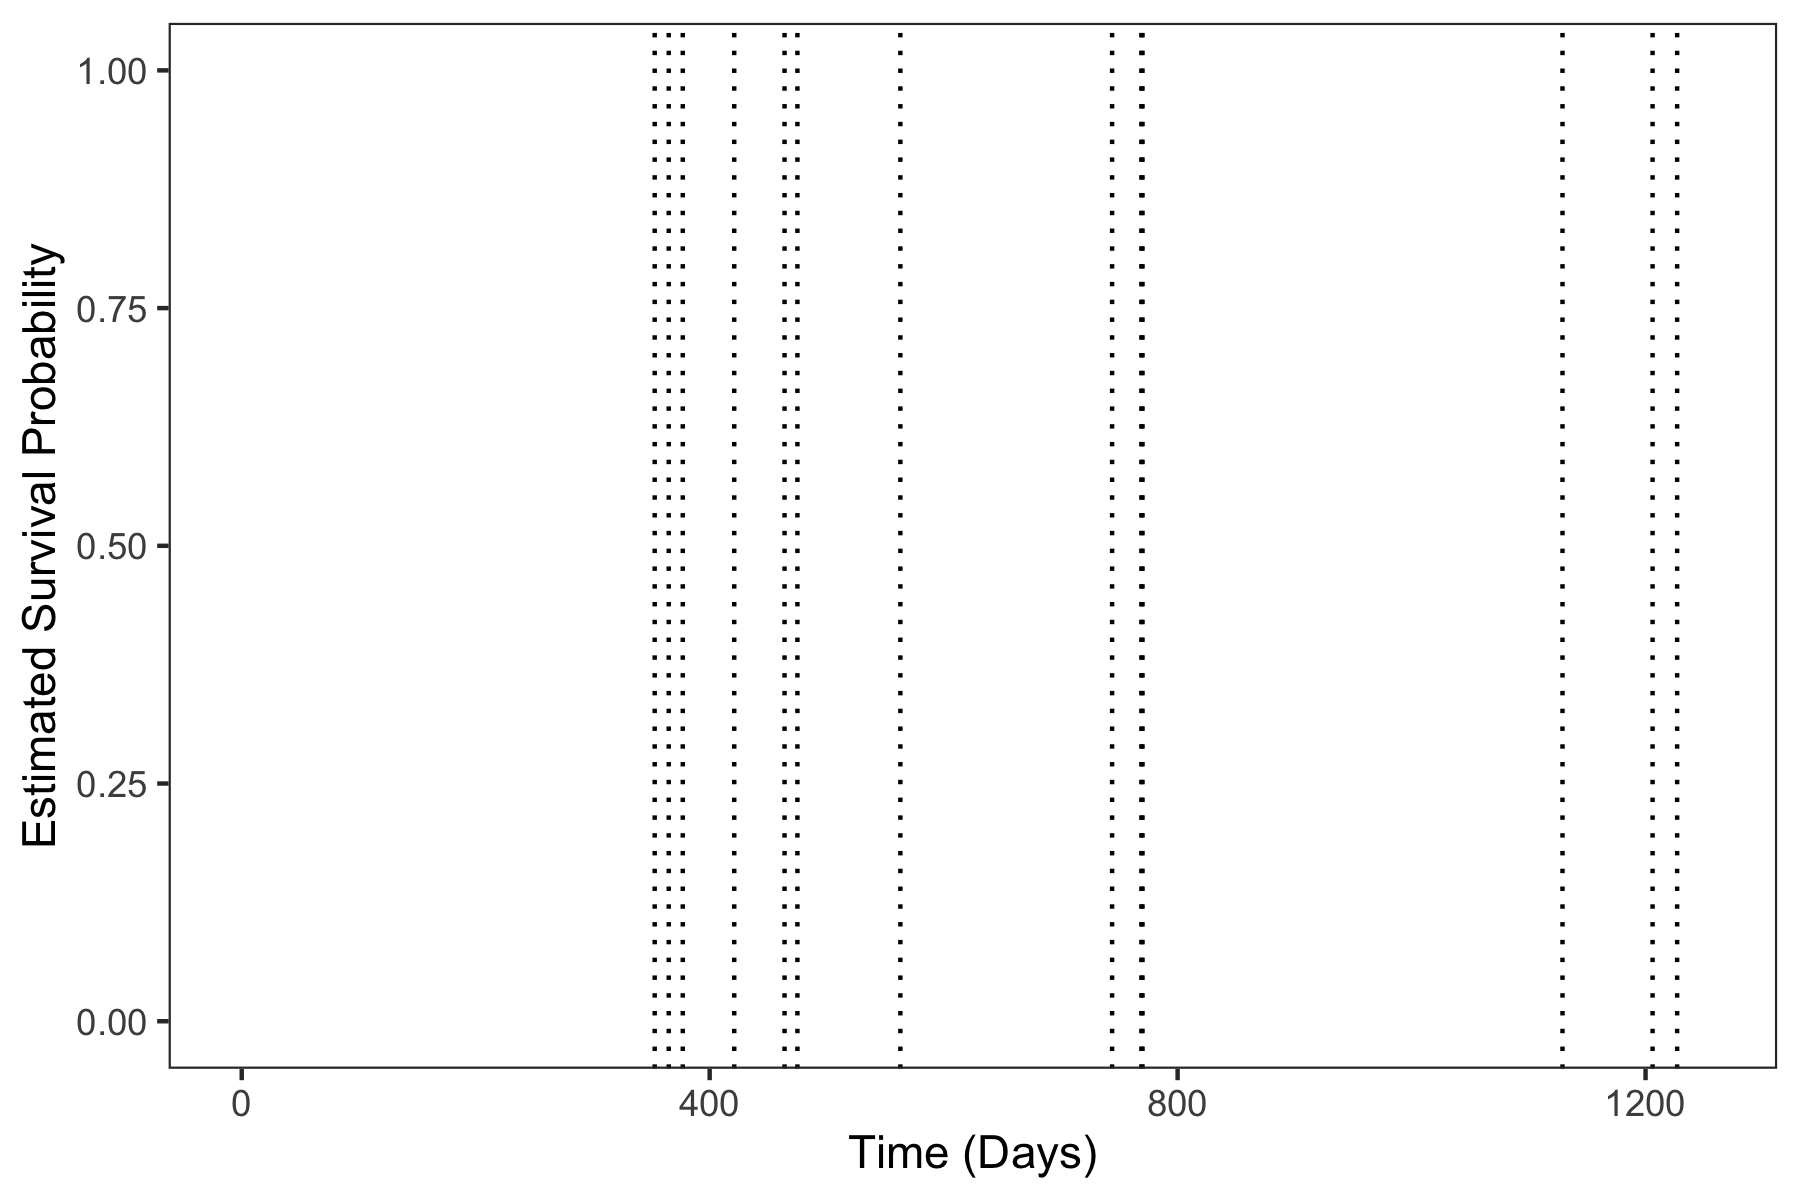
\includegraphics[width=\textwidth]{img/km-curve-sample-rx2.png}
\end{center}
\end{question}

